\section{Outils utilis�s}

\subsection{Environnement de mod�lisation}
\begin{frame}{TopCased}
    \begin{block}{Pr�sentation}
        \begin{itemize}
            \item Analyse d'exigences
            \item Mod�lisation et simulation de mod�les
            \item G�n�ration de code
            \item Application RCP ou plugin Eclipse

        \end{itemize}

    \end{block}

\end{frame}

%

\subsection{R�gles de transformation}
\begin{frame}{ATL Transformation Language}
    \centering
    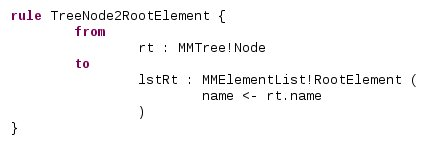
\includegraphics[scale=0.5]{./images/imageATL.jpeg}

    \begin{block}{Pr�sentation}
        \begin{itemize}
            \item Inclus avec TopCased
            \item Langage utilis� dans la transformation de mod�les
            \item Permet d'�crire les correspondances entre 2 �l�ments
            \item R�gles contenant du code OCL

        \end{itemize}

    \end{block}

\end{frame}

%

\subsection{V�rification de compatibilit�}
\begin{frame}{Tool for Interface Compatibility and Composition}
    \centering 
    \begin{columns}
        \begin{column}{0.4\linewidth}
            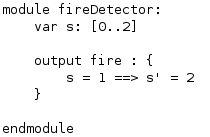
\includegraphics[scale=0.5]{./images/imageTiccParse.jpeg}

        \end{column}

        \begin{column}{0.3\linewidth}
            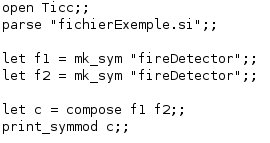
\includegraphics[scale=0.5]{./images/imageTiccExec.jpeg}

        \end{column}

    \end{columns}

    \begin{block}{Pr�sentation}
        \begin{itemize}
            \item Cr�� par notamment par Alfaro
            \item Permet de d�finir des automates d'interface et de les composer 
            \item Poss�de un langage qui lui est propre
            \item Formalise des composants
            \item Utilisation : Un fichier composant .si et un ex�cutable (OCaml) .in

        \end{itemize}

    \end{block}

\end{frame}

